\documentclass [11pt,a4paper]{article}
\usepackage[utf8]{inputenc}
\usepackage[T1]{fontenc}
\usepackage[english]{babel}
\usepackage{textcomp}
\usepackage{lmodern}

% Text Indentation
\usepackage{indentfirst}
\setlength{\parindent}{1cm}

% Section, Subsection & Subsubsection Indentation
\newcommand{\mysection}[1]{
	\setlength{\leftskip}{0cm}
	\section{#1}}
\newcommand{\mysubsection}[1]{
	\setlength{\leftskip}{0.5cm}
	\subsection{#1}}
\newcommand{\mysubsubsection}[1]{
	\setlength{\leftskip}{1cm}
	\subsubsection{#1}}

% Defined header and footer style
\usepackage{fancyhdr}
\pagestyle{fancy}
\renewcommand{\sectionmark}[1]{%
	\markright{\thesection\ #1}}
\fancyhf{}
\fancyhead[LE,RO]{\bfseries\thepage}
\fancyhead[LO]{\bfseries\rightmark}
\fancyhead[RE]{\bfseries\leftmark}
%\lhead{\color{Gray}{\small{Travlendar+ : Manage your Day !}}}
\lfoot{\textcolor{Gray}{\small{Copyright © 2017 Kostandin Caushi, Marcello Bertolini, Raffaele Bongo – All rights reserved}}}
%\rfoot{\textcolor{Gray}{\thepage}}
\renewcommand{\headrulewidth}{1pt}
\fancyhfoffset[lf]{0mm}

% Page margins, header and footer positions
\usepackage{geometry}
\geometry{
	a4paper,
	total={210mm,297mm},
	left=25mm,
	right=25mm,
	top=35mm,
	bottom=25mm,
	headsep=10mm
	}

\interfootnotelinepenalty=10000

% Tables
\usepackage{tabu}
\usepackage{tabularx}
\usepackage{ltablex}
\usepackage{longtable}
\usepackage{float} % To allow the use of H modifier in long tables

% Graphics
\usepackage{graphicx}
\usepackage[dvipsnames, table]{xcolor}

\usepackage{ifthen}
\usepackage{xspace}
\usepackage{enumitem}
\usepackage{amssymb}
\usepackage[pdftex, colorlinks]{hyperref}
\hypersetup{%
	colorlinks = true,
	linkcolor  = black,
	pdfauthor  = {Kostandin Caushi, Marcello Bertolini, Raffaele Bongo},
	pdftitle   = {Travlendar+}
}
\newcommand{\comment}[1]{{\color{Blue}$\blacktriangleright$ Comment: #1 $\blacktriangleleft$}}

\begin{document}
	\begin{titlepage}
		\centering
		%LOGO
		\begin{figure}
			\vspace*{0mm}
			\centering
			
\includegraphics[scale=0.7]{Images/Polimi_Logo}
			\\[3cm]
		\end{figure}		
		\vspace{65mm}
		\textcolor{Blue}{\textbf{\Huge TRAVLENDAR+}}\\[15mm]
		\textcolor{Blue}{\textbf{\huge RASD}}\\[4mm]
		{\textcolor{Blue}{\textbf{\Large{Requirement Analysis and Specification Document}}}}\\
		\vspace{30mm}
		\textit{\large Kostandin Caushi 898749}\\[3mm]
		\textit{\large Marcello Bertolini 827436}\\[3mm]
		\textit{\large Raffaele Bongo 900090}\\[3mm]
		\vspace{30mm}
		Date 05/01/2018\\
		\vspace{10mm}
		Version 3
	\end{titlepage}

%------------------------------
	\begin{center}
	\vspace*{-5mm}
	\renewcommand{\contentsname}{Table of Contents}
	\tableofcontents
	\newpage
	\listoffigures
	\newpage
    \end{center}
	
%-----------------------------
	\ttfamily
	\setlength{\emergencystretch}{45pt}
	\vspace*{-5mm}
\mysection{Introduction}

\mysubsection{Purpose}
This document represents the Requirement Analysis and Specification Document (RASD).
All the goals of the application, the functional and non-functional requirements for achieving them are here reported.\par
There are also the use cases of the system and various scenarios that represent the examples of a real life system’s utilization.
This document is addressed to the developers who have to implement the application’s requirements and it also could be used as a contractual basis.

\mysubsection{Scope}
The system that we will expose in this paper is called Travlendar+. 
Travlendar+ is a calendar-based application that has the aim of managing the many meetings, events and appointments that a user has to deal with every day.\par
After the registration and the login, the system will let the user create events in his personal calendar, checking if he is able to reach them on time and supporting his choices about the way of reaching the location. In fact, the user will be able to insert customizable settings which will allow the system to give him back precise advices about the means of transport, including taxis and sharing services means, to use.\par
Travlendar+ will also give the user the possibility to buy tickets of a town’s public means of transport and it will also allow him to manage his travels to reach other cities, creating specific travel events in the calendar section.
The system will offer other additional features :
\begin{itemize}
	\setlength{\leftskip}{0.5cm}
	\item The possibility to register the season ticket for the public transport. Travlendar+ will notify the user when the expiration date is near.
	\item The possibility to set the starting time, ending time and the preferred duration of every day lunch. The system will guarantee to preserve at least 30 minutes for this purpose.
	\item In case of outdoor trips, the user will be able to insert the period he will spend out of town and the system will suggest him the most convenient public transport tickets available keeping in mind the information given.
	\item The possibility of setting the anticipation time for reaching the various events. The system will warn the user when he needs to leave in order to arrive on time.
\end{itemize}

\newpage
\mysubsection{Definitions}
\begin{itemize}
	\setlength{\leftskip}{0.5cm}
	\item \emph{\textbf{System : }}the software and hardware components that characterize Travlendar’s environment.
	\item \emph{\textbf{Outdoor : }}a different location from the user’s residence town.
	\item \emph{\textbf{Outdoor Transport Service : }}the services dedicated to the transport between different towns.
	\item \emph{\textbf{Local Public Transport Service : }}the services dedicated to the transport within a town.
	\item \emph{\textbf{Event : }}a generic word used for speaking about appointments, meetings, etc. added to the calendar.
	\item \emph{\textbf{Event Path : }}a part of an event solution that the user can perform with a specific mean of transport.
	\item \emph{\textbf{Event Solution : }}a set of event path that allow the user to reach the event location.
	\item \emph{\textbf{Warning : }}the method used by system to warn the user about something.
	\item \emph{\textbf{Best means of transport options : }}the best transport found by the system according to the user’s preferences.
	\item \emph{\textbf{Preferences : }}a set of options that modify the behaviour of the system when computing the routes.
	\item \emph{\textbf{Sharing Means : }}bike or car sharing.
	\item \emph{\textbf{User : }}the person who has performed a registration and is logged in the system.
	\item \emph{\textbf{Anticipation Time : }}it specifies how much time before the beginning of the event the user wants to arrive with.
	\item \emph{\textbf{TAG : }}it’s a collection of information, created by the user, which can be associated to an event and contains the preferred means of transport and anticipation time to use.
	\item \emph{\textbf{Residence : }}the user’s home address.
	\item \emph{\textbf{Accommodation : }}the user’s occasional accommodation address located in a town different from the one reported in his profile.
	\item \emph{\textbf{Trip : }}a set of information about the journey that the user has organized.
	\item \emph{\textbf{Travel event : }}an event that contains all the information about the travel between two different towns such as start time, end time and the mean of transport involved.
\end{itemize}

\mysubsection{Acronyms}
\begin{itemize}
	\setlength{\leftskip}{0.5cm}
	\item \emph{RASD : }Requirement Analysis and Specification Document
	\item \emph{API : }Application Programming Interface
\end{itemize}

\mysubsection{Abbreviations}
\begin{itemize}
	\setlength{\leftskip}{0.5cm}
	\item \lbrack Gn] : Goal n
	\item \lbrack Rn] : Requirement n
	\item \lbrack Dn] : Domain n
\end{itemize}

\mysubsection{Goals}
\begin{itemize}
	\setlength{\leftskip}{0.5cm}
	\item \lbrack G$_{1}$] Allow the user to register and to log into the system.
	\item \lbrack G$_{2}$] Allow user to add events in the calendar.
	\item \lbrack G$_{3}$] Allow the user to receive the mobility options.
	\item \lbrack G$_{4}$] Support the user to avoid getting late on appointment.
	\item \lbrack G$_{5}$] Allow the user to have advices about the means of transport that can minimize his carbon footprint.
	\item \lbrack G$_{6}$] Support the user to have at least 30 minutes of lunch every day.
	\item \lbrack G$_{7}$] Allow the user to buy local public transport ticket.
	\item \lbrack G$_{8}$] Give advice about the best public transportation ticket to buy.
	\item \lbrack G$_{9}$] Remember the user about the expiry date of his season ticket, if he has inserted one.
	\item \lbrack G$_{10}$] Allow the user to buy ticket for outdoor travels.
	\item \lbrack G$_{11}$] Allow the user to use local sharing services.
	\item \lbrack G$_{12}$] Allow the user to set the preferences in the settings section.
	\item \lbrack G$_{13}$] Allow the user to handle his trips.
\end{itemize}

\mysubsection{Reference Documents}
\begin{itemize}
	\setlength{\leftskip}{0.5cm}
	\item Mandatory Project Assignments.pdf
	\item Requirement+Engineering+Part+III.pdf
	\item IEEE standard on requirement engineering.pdf
	\item Paper by Jackson and Zave on the word and the machine.pdf
	\item Software Abstractions -Logic Language and Analysis.\\
	Author: Daniel Jackson
\end{itemize}

\mysubsection{Document Structure}
This paper is composed by 5 chapters :
\begin{enumerate}
	\setlength{\leftskip}{0.5cm}
	\item The first chapter is constituted by an introduction of the system, his application domain, his goals and a glossary with the most common expression used in order to give to the reader a basic knowledge of the system and to make him understand better the subsequent parts.
	\item The second part consists of an overall description of the system and the main functionalities, which are listed and described. It also describes the relation of the system with the external services and how they interact. The constraints that have to be respected in order to use the system properly are also explained.
	Moreover, a classification of the system’s actors and the domain properties are given to the reader.
	\item The third part is composed by the specific requirements identified, both functional and non-functional, some mockups that show the most important features and how the user will be able to interact with the system.
	\item The fourth part is composed by 6 scenarios that describe how the system will work and how it will perform his functionalities.
	\item The fifth and final part is composed entirely by Alloy code and some snapshot of the world generated with the related tool.
\end{enumerate}
	\newpage
	\vspace*{-5mm}
\mysection{Overall Description}

\mysubsection{Product Perspective}
The system, for achieving its goals, will be related with five kind of external components :
\begin{itemize}
	\setlength{\leftskip}{0.5cm}
	\item Root Providers (Google Maps)
	\item Local Transport Services
	\item Outdoor Transport Services
	\item Sharing Services
	\item Environment Service
\end{itemize}
To localize the means and the user’s positions and to retrieve the directions, we will use in our system Google maps API. The system will format the data received in a standardized manner and show them to the user according to his preferences.\par
Our system will contain all the references to the local and outdoor transport services, which APIs will be known in order to retrieve the requested information about the tickets’ prices. 
Once the user has chosen the ticket, he will be addressed to the service’s website to complete the purchase.\par
At first the system will advise about the best local transport tickets only in the towns of Milano, Torino and Rome; for the other towns, the system will give the user the possibility to access to the local transport websites.
Regarding the outdoor travels, it will be possible to buy tickets only with a restricted group of transport services such as Trenitalia and Alitalia.
\begin{figure}[H]
	\centering
	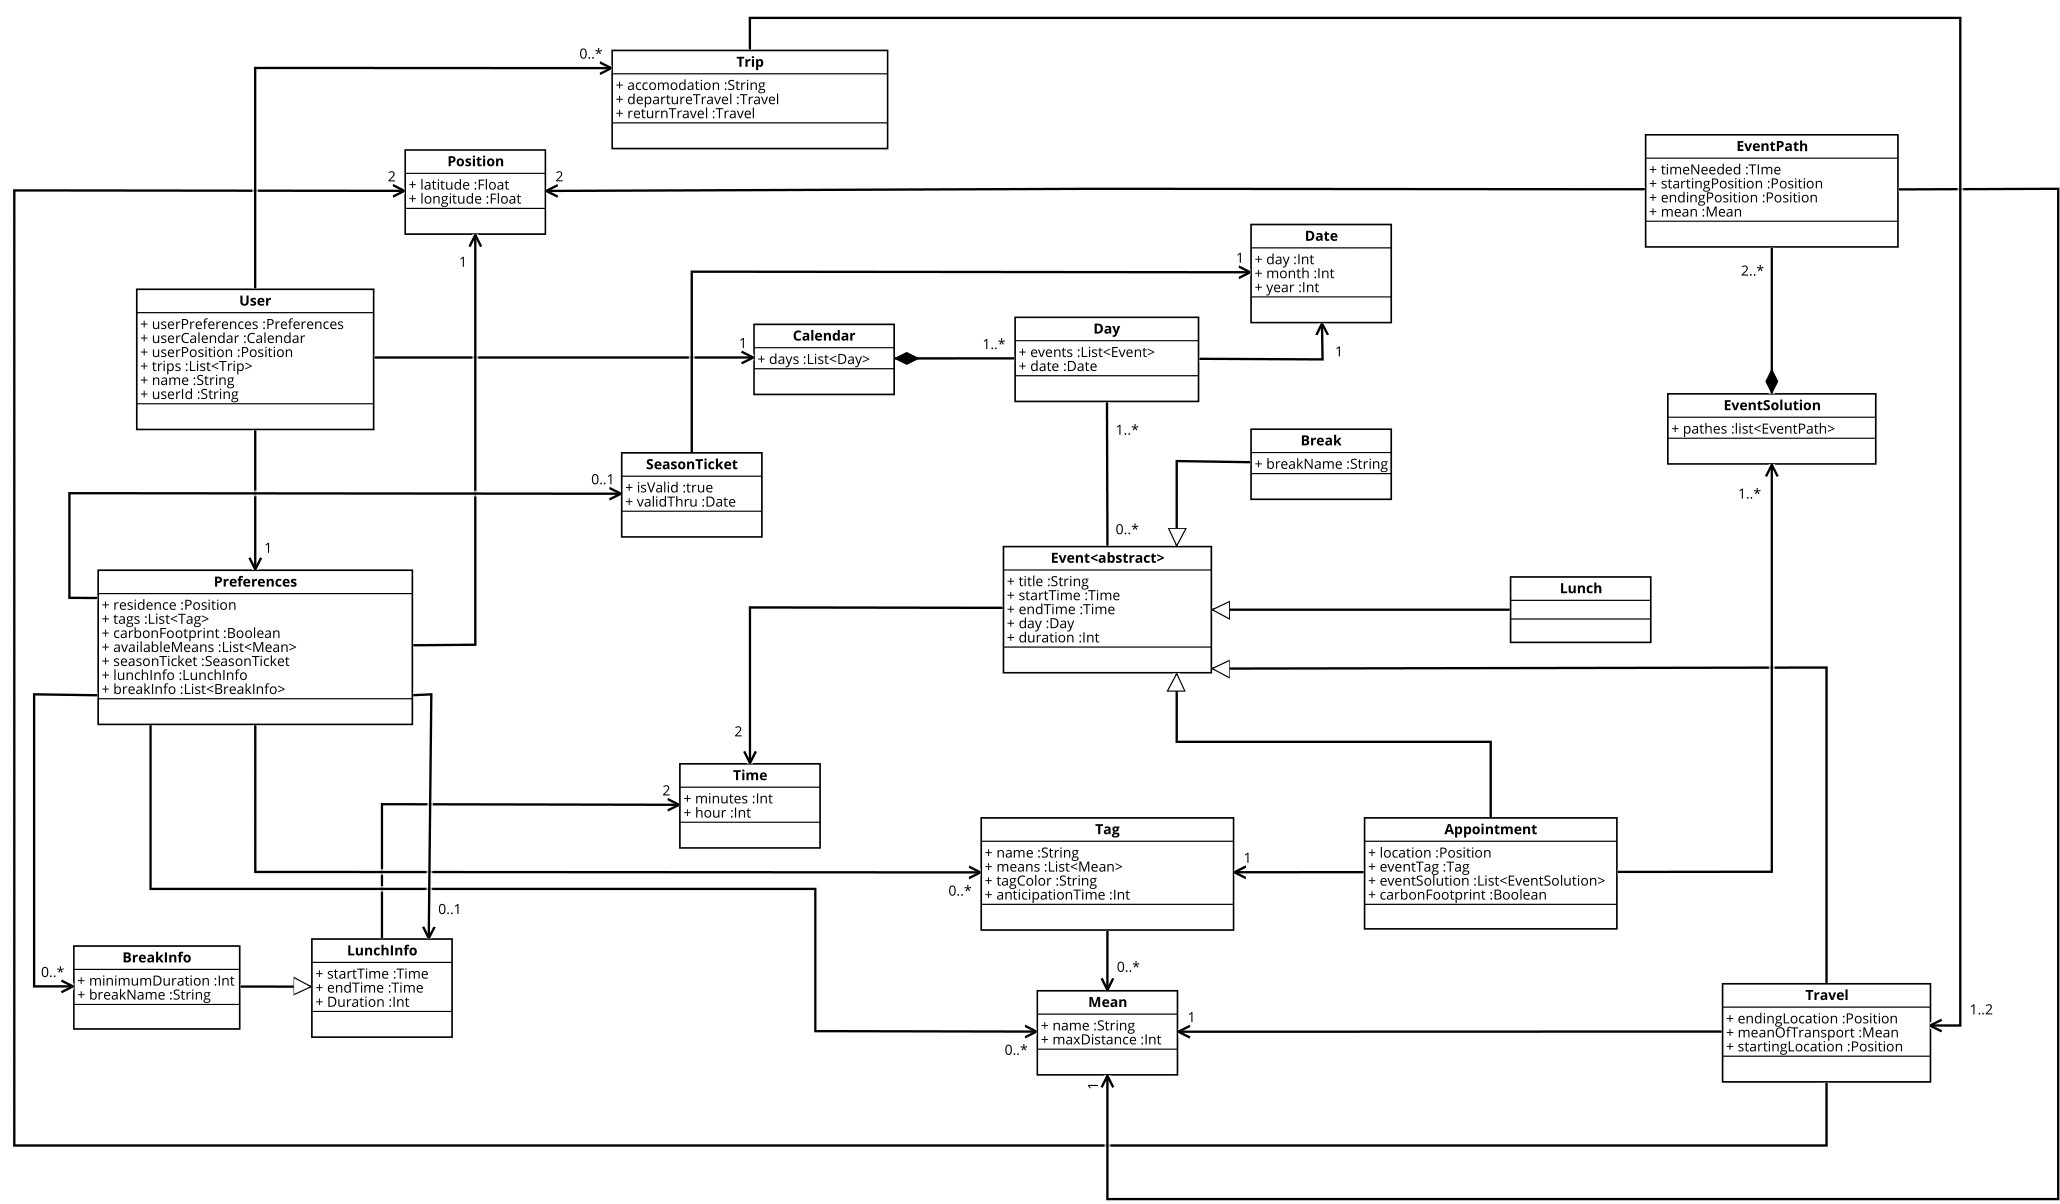
\includegraphics[scale=0.25]{Images/Class_Diagram}
	\caption{Class Diagram}
\end{figure}

\mysubsection{Product Functions}
In order to provide a clear vision of the system’s aims that will be implemented, we are going to show some use cases diagram representing the system’s features. A description of the main ones will be provided.
\begin{figure}[H]
	\centering
	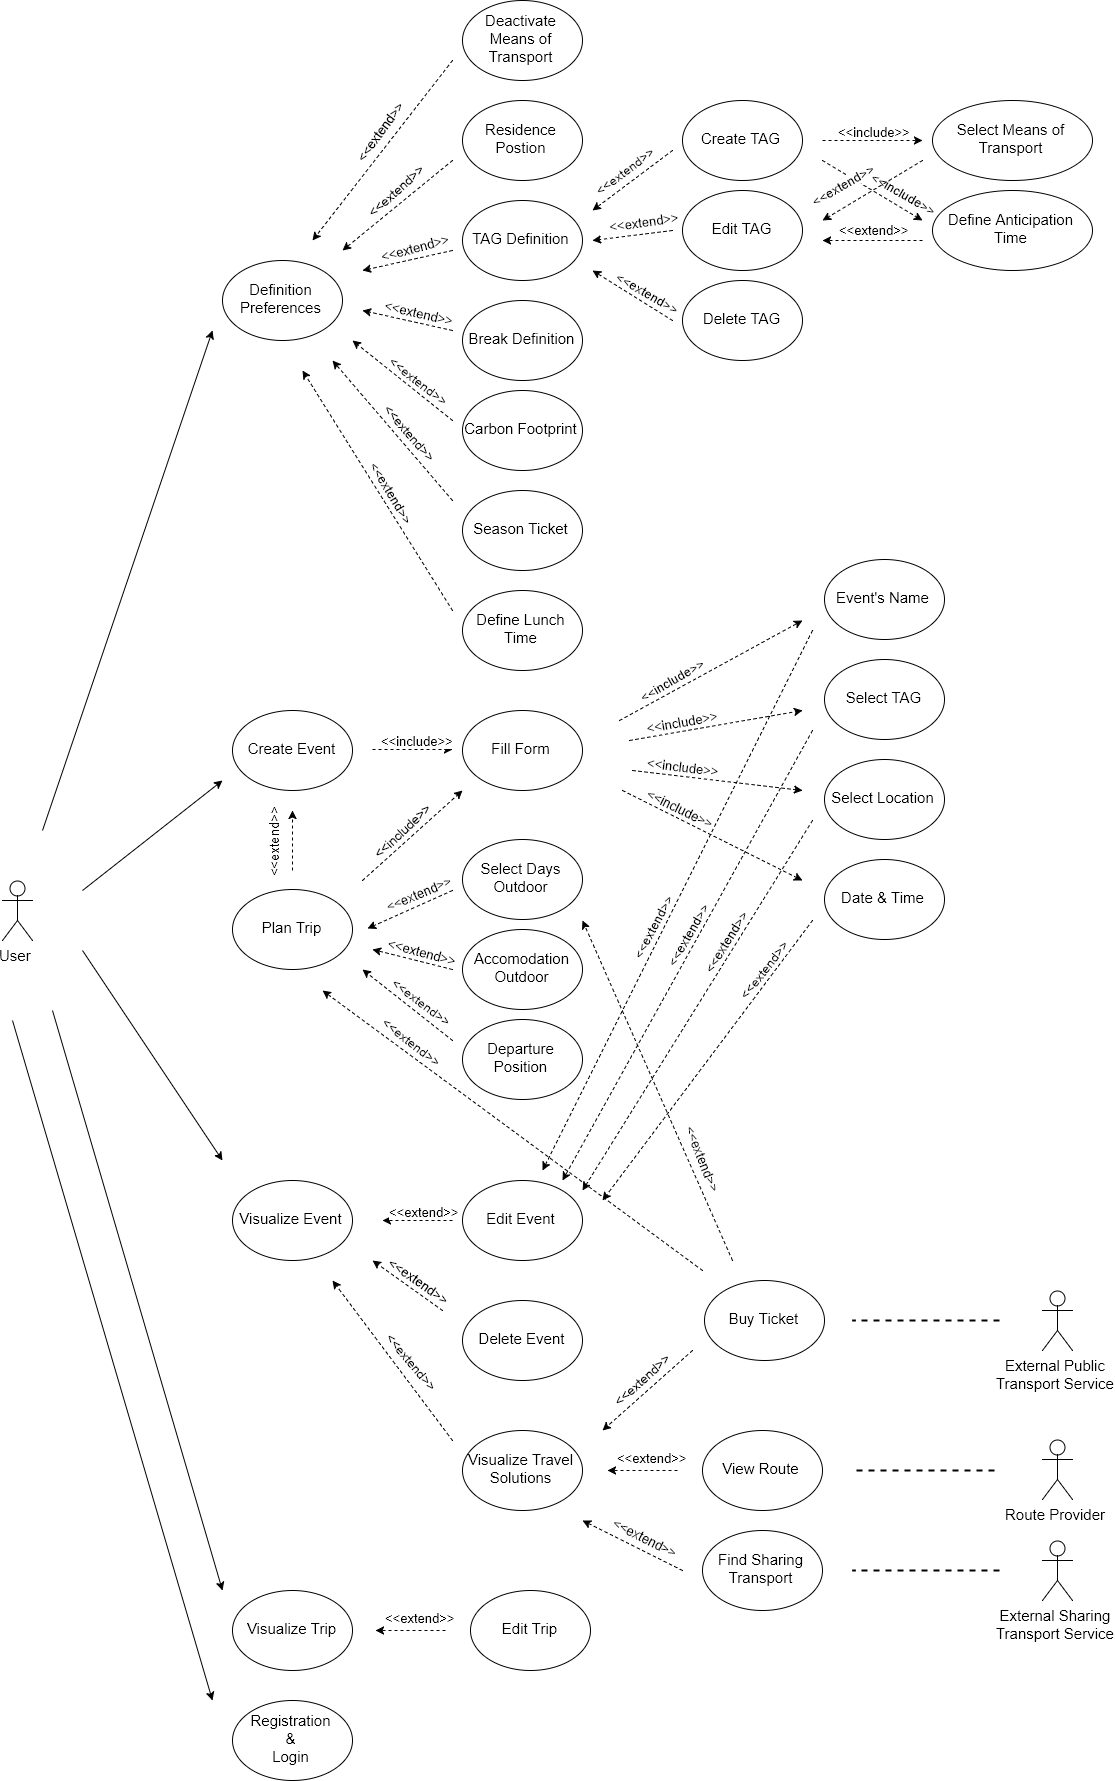
\includegraphics[scale=0.25]{Images/Use_Case/General_Use_Case}
	\caption{General Use Case}
\end{figure}

\mysubsubsection{Registration \& Login}
The system will let the user to sign up, inserting the e-mail and password for creating his personal profile and he will be able to sign-in every time he wants.

\mysubsubsection{Set Preferences}
\begin{figure}[H]
	\centering
	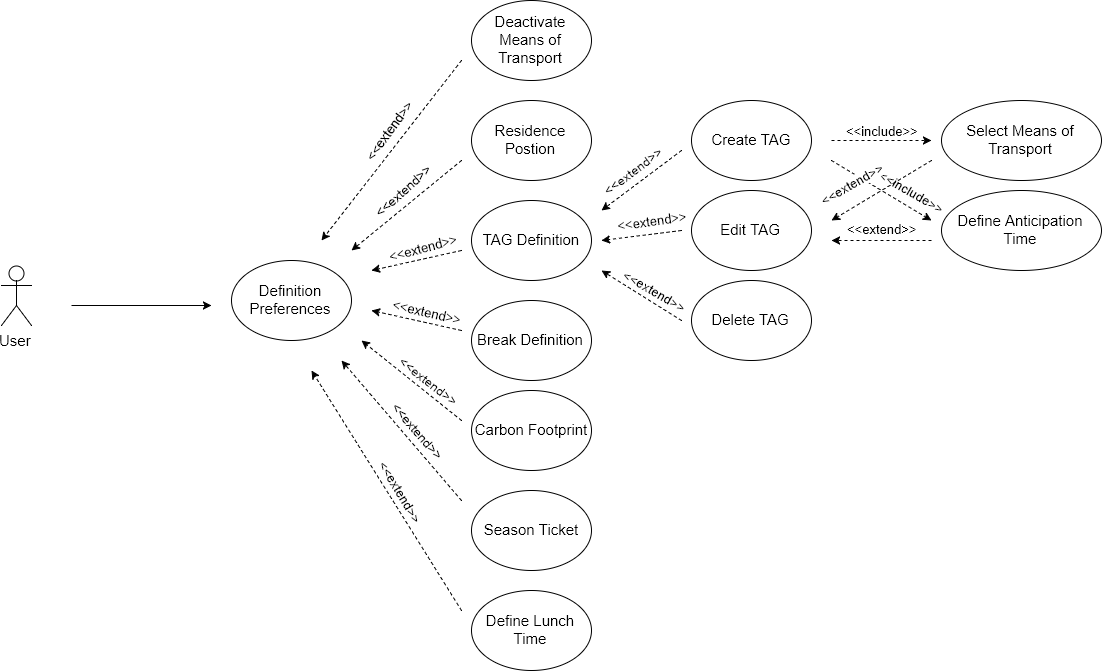
\includegraphics[scale=0.25]{Images/Use_Case/Set_Preferences}
	\caption{Set Preferences Use Case}
\end{figure}
The user will be able to set many preferences to customize his profile. 
He will be able to :
\begin{itemize}
	\setlength{\leftskip}{1cm}
	\item insert his season ticket and receive warnings to remind him the expiry date.
	\item set his home address that will allow the system to compute the routes for reaching the first event of the day using it as the route starting point.
	\item define the means of transport that he never wants to use.
	\item minimize his carbon footprint.
	\item set the constrains about the maximum distance that the user wants to cover with a precise mean of transport.
	\item create and define TAGs.
	\item set the default lunch time window and duration. The duration must be equal or greater than 30 minutes.
	\item define a break time window and its duration, as in the lunch preference, but with the possibility of setting also a minimum duration time.
\end{itemize}\par
A TAG will be used to define the type of the event. It will contain the list of means of transports and the anticipation time for reaching the event associated with.

\newpage
\mysubsubsection{Guarantee at Least 30 Minutes of Lunch Break}
Each lunch event is created automatically considering the time window and duration set in the preference section.\par
The system will guarantee at least 30 minutes of lunch per day. In fact, every time that the user will try to create an event, that overlaps the lunch event, the system will check if it is possible to move the lunch event, keeping the same duration, in the time window defined. If not, the system will check if it’s possible to reduce the default lunch duration guaranteeing the 30 minutes’ constraint. In this case, the system will ask the user if he wants to confirm the changes proposed, otherwise it will not be possible to add the new event.

\mysubsubsection{Add Events to the Calendar}
\begin{figure}[H]
	\centering
	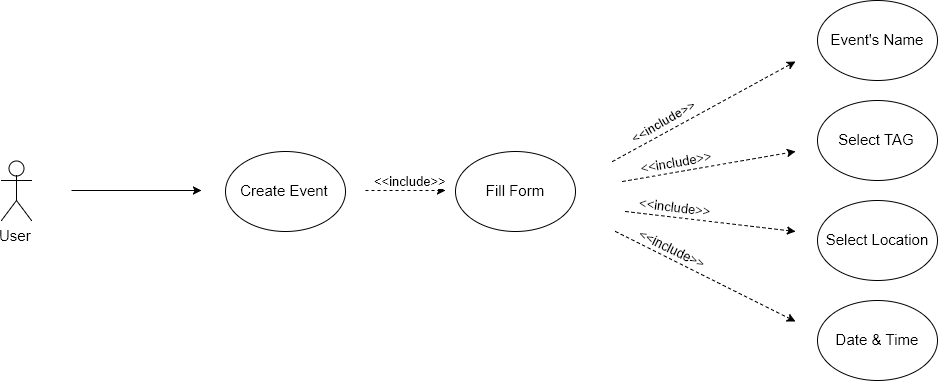
\includegraphics[scale=0.25]{Images/Use_Case/Add_Event}
	\caption{Add Event Use Case}
\end{figure}
The system will let the user add a new event to the calendar.  The user will have to set the title, date and time, carbon footprint preference and must associate the event with a TAG. 
Once done, the system will check if the event is reachable by the previous one, if the next event is reachable from this one and if there’s not overlapping. 
If the three previous conditions are confirmed, the new event will appear in the calendar.

\mysubsubsection{Give Advices About the Means of Transport}
\begin{figure}[H]
	\centering
	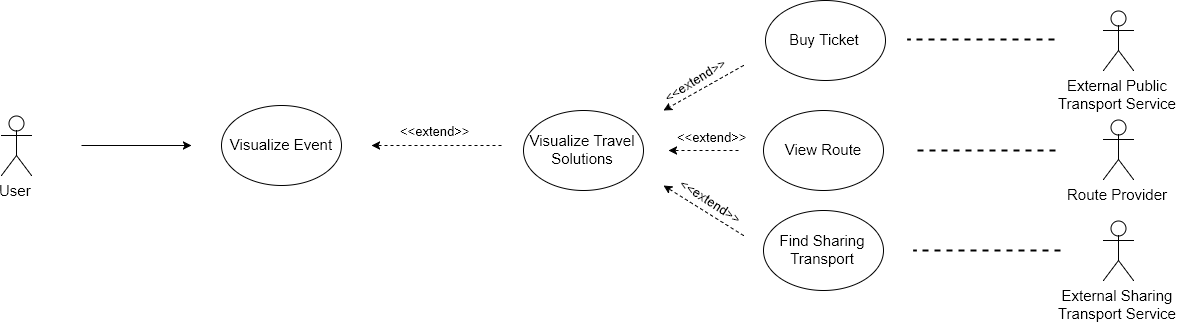
\includegraphics[scale=0.25]{Images/Use_Case/Advice_Mean}
	\caption{Advice Mean, Sharing and Ticket Purchase Use Case}
\end{figure}
The system will show the user the advices about the best means of transport for reaching every event that he has to attend. The routes will be calculated using as starting point :
\begin{itemize}
	\setlength{\leftskip}{1cm}
	\item the previous event as the default option.
	\item the home address/outdoor accommodation if the event to reach is the first one of the day.
	\item the user position.
\end{itemize}\par
In any case, it will be possible to show the directions of every event using as starting point his position, just tapping on a specific button in the map interface.\par
The advices will follow the user’s preferences described in the TAG related to the event, keeping into account also the weather conditions and giving him warnings in the presence of strikes. Moreover, it will be given a warning when the user needs to leave in order to reach the event on time.\par
The system will also localize and show the position of the nearest car and bike sharing services.

\mysubsubsection{The Local Transport Tickets : Recommendation and Purchasing}
The system will recommend and allow to buy the best transport ticket. This feature is available just in the towns reported in the previous section.\par
Furthermore, during the trip management, after having inserted the accommodation address and the duration, the system will give back to the user the tickets available, their prices and the best option that covers the entire period. The user will be able to purchase them after being addressed to the local service website/application. 

\mysubsubsection{Trip Management}
\begin{figure}[H]
	\centering
	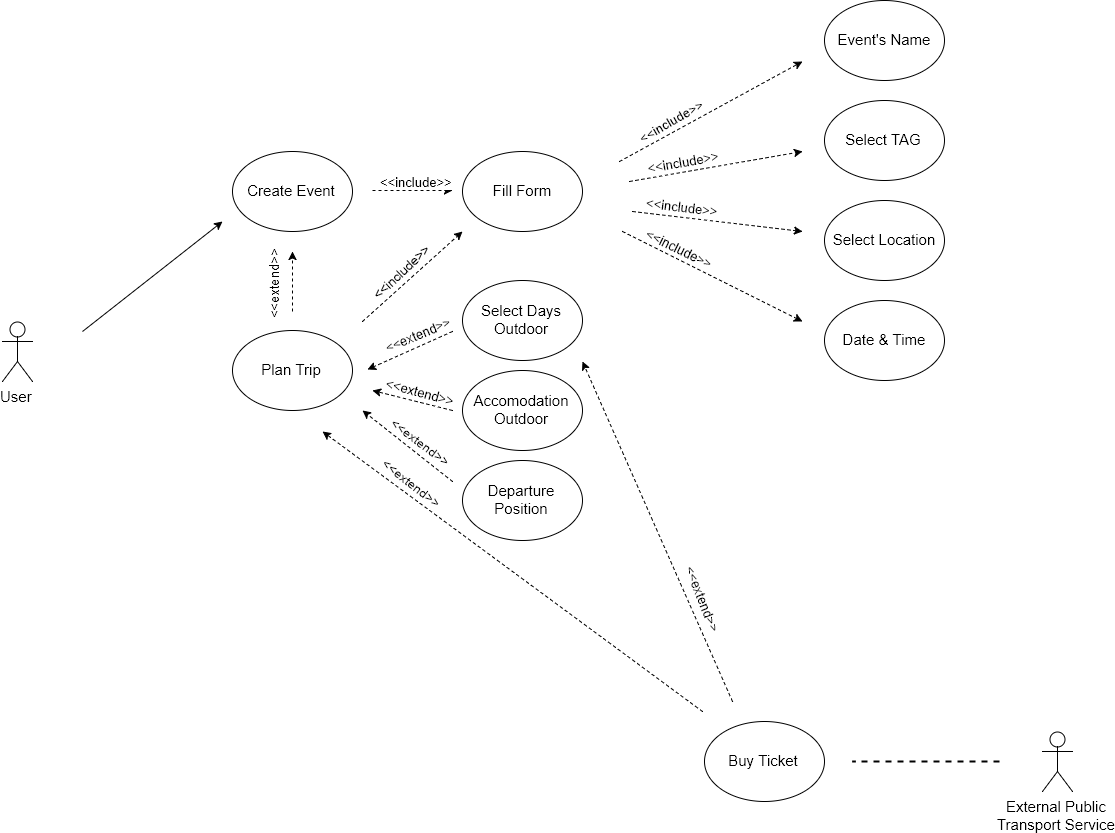
\includegraphics[scale=0.25]{Images/Use_Case/Trip}
	\caption{Trip Management and Ticket Purchase Use Case}
\end{figure}
The system will allow the user to manage trips and, by defining the accommodation and the duration, it will suggest the tickets available for reaching the desired town. It will be possible to arrange a trip directly from the calendar section. Furthermore, when an event is created and it’s located in a town different from the user’s position, the trip’s arrangement will be prompted.\par
The travel will be represented as a special event in the calendar’s section that covers the entire travel time and contains all the information.
The user will be able to edit the trip information any time he wants, accessing the trips section.

\mysubsection{User Characteristics}
The system is suitable for any kind of user. In fact, the Travlendar+ goals are appropriate for any person who needs help for taking on the everyday organization.\\
\par
\emph{\textbf{Actors}}
\begin{itemize}
	\setlength{\leftskip}{1cm}
	\item \emph{\textbf{User : }}is a person who has done the subscription in the system. Every user, after the login process, is able to use all the system’s functionalities.

	\item \emph{\textbf{System Manager Team : }}it’s a group of engineers and programmers to whom the founders have entrusted the maintenance of the system and its upgrade for answering promptly to the users’ needs.

	\item \emph{\textbf{Client Service : }}it is a small team that has the aim of receiving and resolving users’ complaints and requests.
\end{itemize}

\mysubsection{Domanin Properties}
\begin{enumerate}
	\setlength{\leftskip}{1cm}
	\item User id must be unique.
	\item GPS position is always correct.
	\item GPS cannot be switched off.
	\item Event creation implies the user’s participation to it.
	\item Events do not overlap with each other.
	\item Every event in the calendar is reachable from the previous one.
	\item The duration of the event in the world corresponds to the duration of the one in the calendar.
	\item Only the user can create, edit and delete the event in his calendar.
	\item Public transports respect the timetables.
	\item The means of transport suggested are actual available.
	\item Every user has one calendar.
	\item External transport services always answer to the system requests.
	\item The user has to create the event before it starts.
	\item Subways, Trams and bikes do not emit CO2.
	\item Each local transport mean belongs to its transport service.
	\item User can be just in one position at a time.
	\item The weather forecasts are always reliable.
	\item External services answer to the system request in no more than 5 seconds.
	\item The user who asks to purchase a ticket on the system, will actually buy the ticket in the  transport system external service.
	\item Means of transport are composed by: buses, subways, trams and trains.
\end{enumerate}
	\newpage
	\vspace*{-5mm}
\mysection{Specific Requirements}

\mysubsection{Proposed System}

\mysubsection{External Interface Requirements}

\mysubsubsection{User Interfaces}
The following mockups represent an idea of the interfaces that will be provided to the user.

\mysubsection{Functional Requirements}
\vspace{0.5cm}
\noindent
\emph{\textbf{[G$_{1}$] : Allow the user to register and log into the system}}
\begin{itemize}
	\setlength{\leftskip}{0.5cm}
	\item \lbrack R$_{1}$] : The System has to check the credentials.
	\item \lbrack R$_{2}$] : A registered user must be able to log in the system.
\end{itemize}

\vspace{0.5cm}
\noindent
\emph{\textbf{[G$_{2}$] : Allow the user to add events in the calendar}}
\begin{itemize}
	\setlength{\leftskip}{0.5cm}
	\item \lbrack R$_{1}$] : The system mustn’t allow events overlapping.
	\item \lbrack R$_{2}$] : The system has to guarantee the minimum lunch duration.
	\item \lbrack R$_{3}$] : The system has to give the possibility to the user of arriving on time to the new event.
	\item \lbrack R$_{4}$] : The system has to be able to add the new event to the calendar.
\end{itemize}

\vspace{0.5cm}
\noindent
\emph{\textbf{[G$_{3}$] : Allow user to receive the mobility options}}
\begin{itemize}
	\setlength{\leftskip}{0.5cm}
	\item \lbrack R$_{1}$] : The system has to check that the event has been created.
	\item \lbrack R$_{2}$] : The system is able to communicate with the route provider.
	\item \lbrack R$_{3}$] : The system sends data about the starting and ending location to the route provider.
	\item \lbrack R$_{4}$] : The system receives the path and the available transport from the external service.
	\item \lbrack R$_{5}$] : The system has to use the information given in the event’s TAG to filter the possible means of transport.
	\item \lbrack R$_{6}$] : The system has to check the travel means enabled by the user.
	\item \lbrack R$_{7}$] : The system has to obey the constraints set by the user about the travel means.
	\item \lbrack R$_{8}$] : The system has to check if the Carbon footprint preference has been enabled.
	\item \lbrack R$_{9}$] : The system has to retrieve user position.
	\item \lbrack R$_{10}$] : The system has to check the weather forecast.
	\item \lbrack R$_{11}$] : The system has to retrieve the appointment location.
	\item \lbrack R$_{12}$] : The system has to know how to show the solution found.
\end{itemize}

\vspace{0.5cm}
\noindent
\emph{\textbf{[G$_{4}$] : Support the user to avoid getting late on appointment}}
\begin{itemize}
	\setlength{\leftskip}{0.5cm}
	\item \lbrack R$_{1}$] : The system has to retrieve the user GPS position.
	\item \lbrack R$_{2}$] : The system has to know how to send warnings to the user.
	\item \lbrack R$_{3}$] : The system has to check the destination position.
	\item \lbrack R$_{4}$] : The system has to check the possibility of reaching on time the next event with the slowest mean of transport in the list of suggested ones.
\end{itemize}

\vspace{0.5cm}
\noindent
\emph{\textbf{[G$_{5}$] : Allow the user to have advices about the means of transport that can minimize his carbon footprint}}
\begin{itemize}
	\setlength{\leftskip}{0.5cm}
	\item \lbrack R$_{1}$] : The system must be able to check the carbon footprint preference.
	\item \lbrack R$_{2}$] : The system must know how to filter the means of transport to minimize their carbon footprint.
\end{itemize}

\vspace{0.5cm}
\noindent
\emph{\textbf{[G$_{6}$] : Support the user to have at least 30 minutes of lunch every day}}
\begin{itemize}
	\setlength{\leftskip}{0.5cm}
	\item \lbrack R$_{1}$] : The system must be able to check the lunch preferences.
	\item \lbrack R$_{2}$] : The system must be able to create every day a lunch based on the user preferences.
	\item \lbrack R$_{3}$] : The system must be able to avoid the creation of those events that prevent the presence of a lunch with the minimum duration.
\end{itemize}

\vspace{0.5cm}
\noindent
\emph{\textbf{[G$_{7}$] : Allow the user to buy local transport ticket}}
\begin{itemize}
	\setlength{\leftskip}{0.5cm}
	\item \lbrack R$_{1}$] : The system has to check that all the necessary travel info have been inserted by the user.
	\item \lbrack R$_{2}$] : The system has to address the user to the web site/application to complete the ticket purchase.
\end{itemize}

\vspace{0.5cm}
\noindent
\emph{\textbf{[G$_{8}$] : Give advice about the best public transportation ticket to buy}}
\begin{itemize}
	\setlength{\leftskip}{0.5cm}
	\item \lbrack R$_{1}$] : The system has to know how much time the user will stay in town.
	\item \lbrack R$_{2}$] : The system has to be able to get information about tickets from the public transport service.
	\item \lbrack R$_{3}$] : The system has to be able to interpret and elaborate the information received.
	\item \lbrack R$_{4}$] : The system has to find the most convenient ticket.
	\item \lbrack R$_{5}$] : The system has to be able to show the results.
\end{itemize}

\vspace{0.5cm}
\noindent
\emph{\textbf{[G$_{9}$] : Remember the user about the expiry date of his season ticket, if he has inserted one}}
\begin{itemize}
	\setlength{\leftskip}{0.5cm}
	\item \lbrack R$_{1}$] : The system has to check the season ticket’s expiry date.
	\item \lbrack R$_{2}$] : The system has to be able to notify the user that his season ticket is expiring.
\end{itemize}

\vspace{0.5cm}
\noindent
\emph{\textbf{[G$_{10}$] : Allow the user to buy ticket for outdoor travels}}
\begin{itemize}
	\setlength{\leftskip}{0.5cm}
	\item \lbrack R$_{1}$] : The system must check the data inserted by the user to buy the ticket.
	\item \lbrack R$_{2}$] : The system must be able to send the data to the external transport service.
	\item \lbrack R$_{3}$] : The system has to be able to interpret and elaborate the information received.
\end{itemize}

\vspace{0.5cm}
\noindent
\emph{\textbf{[G$_{11}$] : Allow user to use local sharing services}}
\begin{itemize}
	\setlength{\leftskip}{0.5cm}
	\item \lbrack R$_{1}$] : The system has to retrieve the sharing means’ location.
	\item \lbrack R$_{2}$] : The system has to check the user location.
	\item \lbrack R$_{3}$] : The system has to be able to show the sharing mean position to user.
	\item \lbrack R$_{4}$] : The system has to be able to redirect the user to the external sharing service system for booking the mean.
\end{itemize}

\vspace{0.5cm}
\noindent
\emph{\textbf{[G$_{12}$] : Allow the user to set the preferences in the settings section}}
\begin{itemize}
	\setlength{\leftskip}{0.5cm}
	\item \lbrack R$_{1}$] : The system must be able to show the user the possible preferences.
	\item \lbrack R$_{2}$] : The system has to register these preferences in its database.
	\item \lbrack R$_{3}$] : The system has to have access to these preferences each time is needed.
\end{itemize}

\vspace{0.5cm}
\noindent
\emph{\textbf{[G$_{13}$] : Allow the user to handle his trips}}
\begin{itemize}
	\setlength{\leftskip}{0.5cm}
	\item \lbrack R$_{1}$] : The system has to be able to create Travel events.
	\item \lbrack R$_{2}$] : The system has to be able to show the list trips created.
	\item \lbrack R$_{3}$] : The system has to be able to let the user modify the trips when needed.
	\item \lbrack R$_{4}$] : The system has to be able to check the trip’s data.
\end{itemize}
	\newpage
	\mysection{Scenarios}

\mysubsection{Scenario 1}
Giuseppe is an employee of a society. One night, before going to sleep, he receives a call from his chief that inform him that he has to attend three meetings in three different zone of Milan. The next day the chief needs to know if Giuseppe can take part at all these meetings or if he has to ask to someone else. Giuseppe has never been in those zones of Milan and, at the moment, he doesn’t have his car because it’s broken. Thus, he has to find another solution. 
In that moment an idea came in Giuseppe’s mind! He opened the Travlendar+ app on his smartphone and inserted the three events in the calendar using a TAG called \emph{no car}, which was specifically created for this situation. This tag includes all the means of transport supported by the app except the car. During the creation of the last event, Travlendar+ has showed to Giuseppe a warning telling him that the event was unreachable in time from the previous one he set. Knowing this information, Giuseppe called his chief for telling him that he has to ask to someone else just for the third event and that he can attend the first two without any problems because he will take the means suggested by Travlendar+.

\mysubsection{Scenario 2}
Michela is a very busy person and she cares about the environment. She has been very happy to download Travlendar+ on her smartphone because it can suggest the means of transport that have the less impact on the environment. Thus, every day Michela inserts her events in Travlendar+ and she associates to each one the \emph{CO$_2$ free} preference. In this way, the system gives her the information about all the means of transport available for reaching the destination, order by the one who produce the less CO$_2$ quantity to the one who produce the most. This is very useful for Michela, because now she can both follow her wish of having a good impact on the environment and avoid arriving late to her appointments, finding always a good compromise without any difficulties.

\mysubsection{Scenario 3}
Luca lives in Milan and the 20$^{th}$ of October he has a work meeting in Turin. He decides to insert the meeting in his calendar. As soon as he sets all the data defining the event and concludes the creation, a message appears saying that the event is very far and advices Luca to plan a trip. Luca is very happy of having this opportunity and proceeds on. Travlendar+ provides him an interface in which he can chose of buying a ticket for the train or for the airplane or simply adding a travel event with that mean. Luca selects the train, then Travlendar+ asks Luca to fill up a form containing the date and the time in which he would like to leave, in order to provide him all the solutions with the related starting prices. After a quick look, thanks to the ad-hoc filtration of the trains, Luca is able to choose the most suitable ticket. As soon as he decides to purchase it, two things happen: 
\begin{itemize}
	\setlength{\leftskip}{0.5cm}
	\item a travel event with all the information is automatically created;
	\item Luca is addressed on the travel service website to complete the purchase.
\end{itemize}
Luca will be able to check the solutions for arriving to the station on time in every moment tapping on the travel event auto-generated.
When Luca returns on the application, he inserts the period of staying and his accommodation in Turin. After this Travlendar+ advices him to buy the ticket that represents the best compromise between price and utility. Anyway, it also shows him the other possible tickets he can buy.

\mysubsection{Scenario 4}
Sean lives in Milan and he has to attend a work-lunch in Rome tomorrow. He has already the ticket for reaching Rome, because his company has already bought it. Thus, he wants to add the travel event in Travlendar+. Nothing of more simple! Sean has only to tap for about one second the screen on the calendar interface and two choices will appear on the screen: \emph{create an event} and \emph{plan a trip}. Tapping on plan a trip, Travlendar+ will show to Sean an interface in which he can chose the mean of transport and, after this, he can simply insert all the info of his ticket and create the travel event tapping on \emph{Add}.

\mysubsection{Scenario 5}
Gianluca is a financial expert, he has always many meetings during the day and sometimes he forgets to take a break. He needs something which reminds him to reserve some time for having lunch. Travlendar+ is the perfect solution to his needs. Gianluca set in the preferences the span of time in which he wants to have lunch, from 12 to 14, and the preferred duration, 60 minutes. 
Today Gianluca has to add to his calendar one event from 12:00 to 13:00 and another one from 13:30 to 15:00. Travlendar+, given the Gianluca’s setting for the lunch, has already automatically created an event lunch every day between from 12:00 and 13.00. When Gianluca adds the first event, the lunch break slides automatically and covers the period between 13.00 and 14.00 without giving any problems. When the second event was added, some problems came up! In fact, Gianluca will not be able to have a lunch of 60 minute. Despite this, Travlendar+ must reserve at least 30 minutes to lunch per day to each user, so it asks Gianluca if he wants to reduce his lunch time to 30 minutes or postpone the event. Gianluca cannot postpone the event, so he decides of reducing his lunch duration to 30 minutes for tomorrow, leaving the other lunch events unchanged.

\mysubsection{Scenario 6}
Gabriele has inserted in his Travlendar+ application his girlfriend tonight’s party event but he has completely forgotten about it. Fortunately, Travlendar+ sends him warnings to remind him to go to the event whenever the time for reaching the party’s location, without arriving late, with the slowest mean of transport in the list is going to expire. But during almost all these warnings Gabriele was sleeping and he did not read them. He just gets the last one, which advices him to use the car. Unfortunately, Gabriele doesn’t have a car in Milan but he has the drive licence and so he can take a car sharing. Travlendar+ is perfect for Gabriele’s situation! In fact, when he taps on the car choice, the app opens an interface that asks Gabriele to choose between his own car and a car sharing. Choosing the second one, Gabriele is able to see the route for reaching the nearest car location and he can also be addressed to the car sharing service app to book it and reaching his girlfriend party’s location on time. Travlendar+ will also show him the fastest route to reach his destination.
	\newpage
	\mysection{Alloy}
\mysubsection{Code}
\lstinputlisting[language=alloy]{Files/Alloy/Alloy_Travlendar.als}

\newpage
\mysubsection{Run \& Check}
\begin{figure}[H]
	\centering
	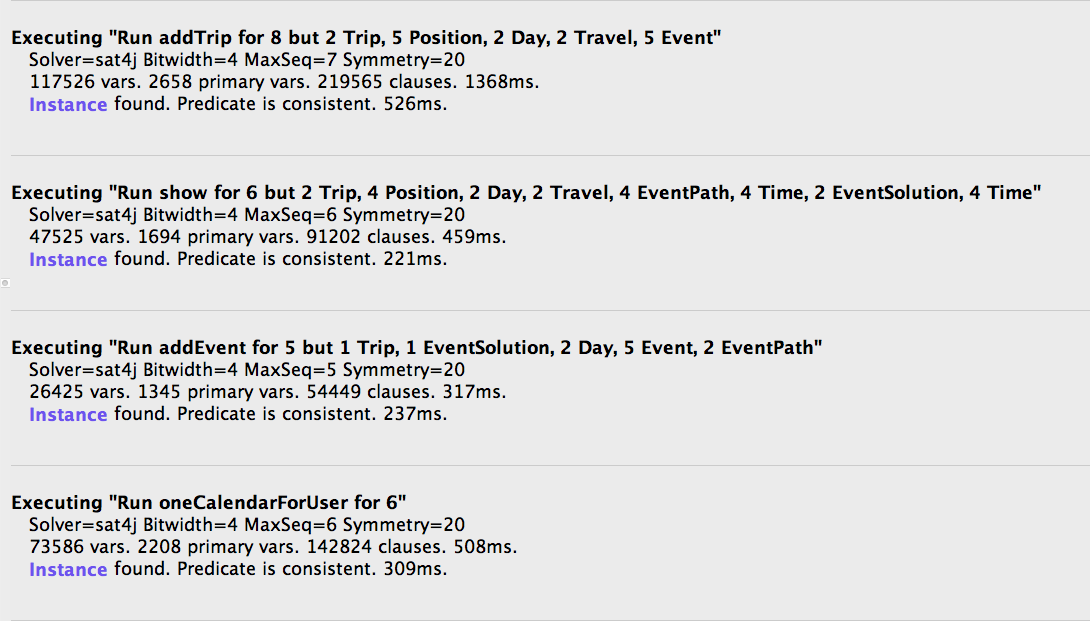
\includegraphics[scale=0.35]{Images/Alloy/Run}
	\caption{Alloy Run Snapshot}
\end{figure}
\begin{figure}[H]
\centering
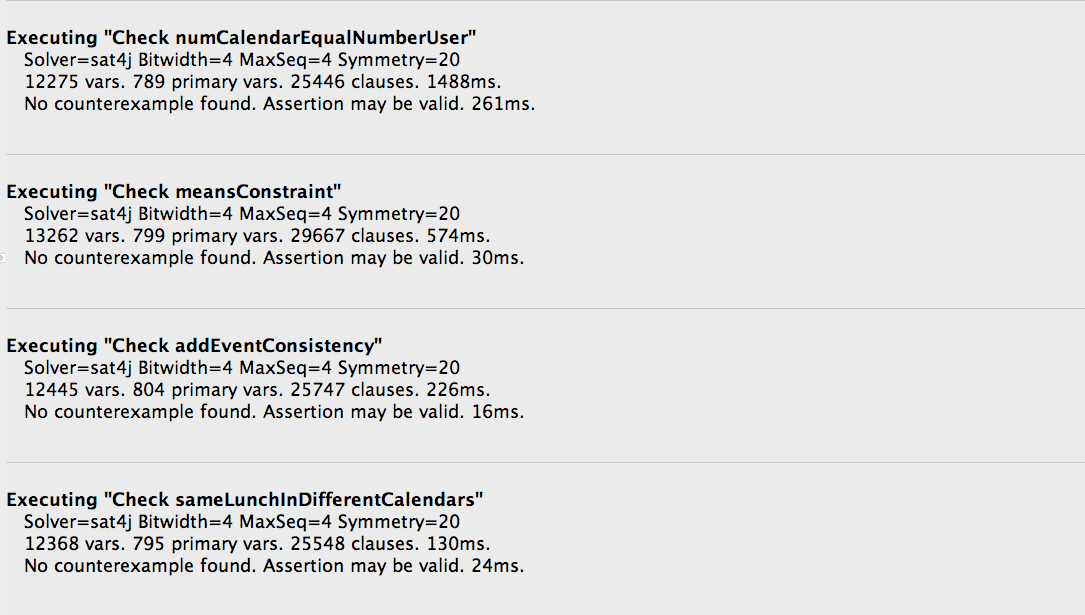
\includegraphics[scale=0.35]{Images/Alloy/Check}
\caption{Alloy Check Snapshot}
\end{figure}

\newpage
\mysubsection{Alloy World}
\begin{figure}[H]
	\centering
	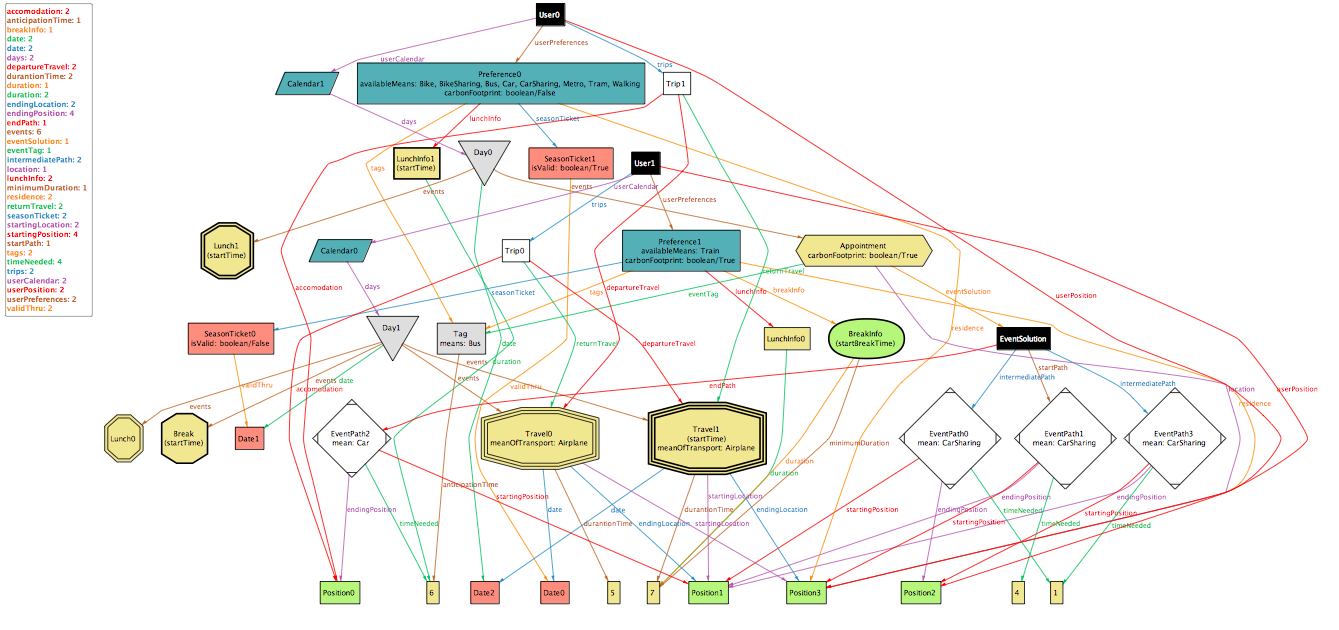
\includegraphics[scale=0.35]{Images/Alloy/Show}
	\caption{Alloy World Snapshot}
\end{figure}

\mysubsection{Alloy Add Event}
\begin{figure}[H]
	\centering
	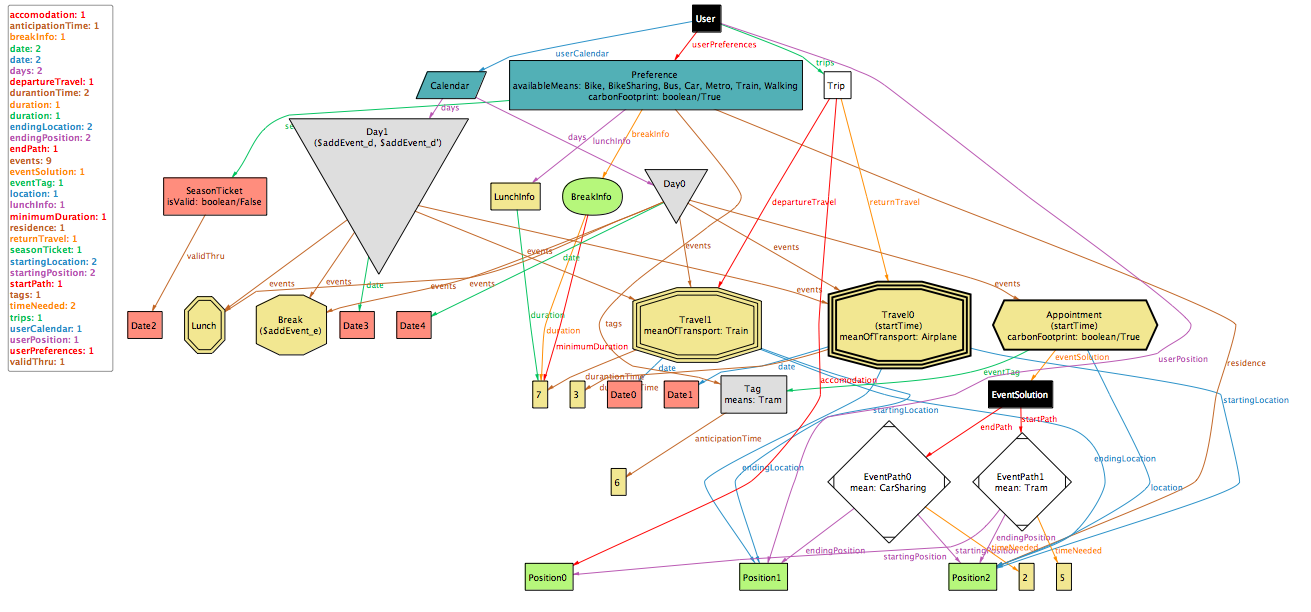
\includegraphics[scale=0.35]{Images/Alloy/Add_Event}
	\caption{Alloy Add Event Snapshot}
\end{figure}

\newpage
\mysubsection{Alloy Add Trip}
\begin{figure}[H]
	\centering
	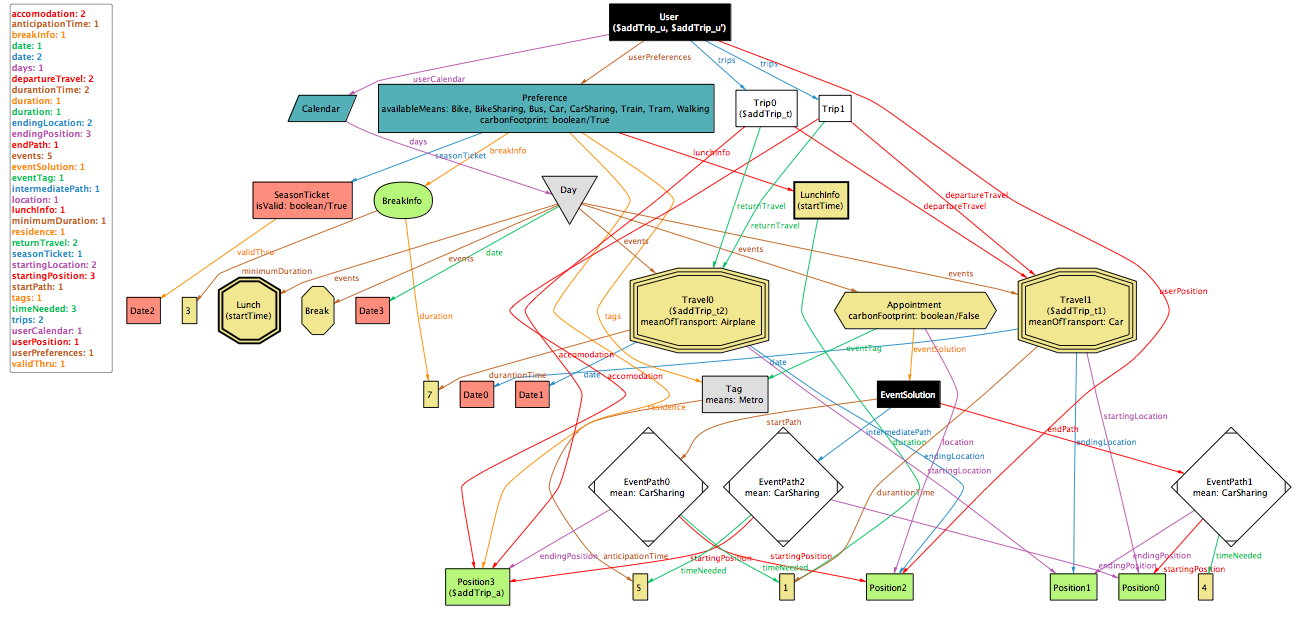
\includegraphics[scale=0.35]{Images/Alloy/Add_Trip}
	\caption{Alloy Add Trip Snapshot}
\end{figure}
	\newpage
	\mysection{Programs Used}
\begin{itemize}
	\setlength{\leftskip}{1cm}
	\item LaTeX TeXstudio : LaTeX Document
	\item Draw.io : Use Cases, Sequence and Activity Diagrams
	\item Signavio : Class Diagram
	\item Sketch : App Mockups
	\item Alloy Analyzer : Alloy
\end{itemize}

\mysection{Revision History}
\vspace{0.5cm}
\begin{tabular}[H]{c|c|c|c}
	Version & Date & Description & Notes\\
	\hline
	\rule{0pt}{4ex}1.0	&	29-10-2017	&	Final Draft	&	-\\
	\rule{0pt}{4ex}1.1	&	30-11-2017	&	Update	&	Architecture and Activity Diagram
\end{tabular}
\vspace{0.5cm}\\

\mysection{Effort Spent}
\mysubsection{Kostandin Caushi}
\vspace{0.5cm}
\begin{tabular}[H]{cc}
	Date & Hours\\
	\hline\\
	06.10	&	2h\\
	07.10	&	2h\\
	08.10	&	4h30\\
	09.10	&	4h\\
	10.10	&	4h\\
	12.10	&	2h\\
	16.10	&	5h30\\
	17.10	&	6h30\\
	19.10	&	4h30\\
	20.10	&	2h30\\
	21.10	&	4h\\
	22.10	&	5h30\\
	23.10	&	2h30\\
	24.10	&	3h30\\
	25.10	&	3h\\
	26.10	&	4h30\\
	27.10	&	6h\\
	28.10	&	4h\\
	29.10	&	4h
\end{tabular}

\newpage
\mysubsection{Marcello Bertolini}
\vspace{0.5cm}
\begin{tabular}[H]{cc}
	Date & Hours\\
	\hline\\
	08.10	&	3h\\
	09.10	&	4h\\
	10.10	&	4h\\
	11.10	&	2h\\
	12.10	&	3h\\
	14.10	&	2h\\
	15.10	&	4h\\
	16.10	&	3h\\
	17.10	&	5h\\
	18.10	&	2h\\
	19.10	&	2h30\\
	21.10	&	2h\\
	22.10	&	2h\\
	23.10	&	2h30\\
	24.10	&	3h30\\
	26.10	&	3h30\\
	27.10	&	2h
\end{tabular}

\mysubsection{Raffaele Bongo}
\vspace{0.5cm}
\begin{tabular}[H]{cc}
	Date & Hours\\
	\hline\\
	07.10	&	2h\\
	08.10	&	3h\\
	09.10	&	4h\\
	10.10	&	4h\\
	14.10	&	5h\\
	15.10	&	2h\\
	16.10	&	3h\\
	17.10	&	5h\\
	19.10	&	3h30\\
	21.10	&	3h\\
	22.10	&	3h\\
	23.10	&	2h30\\
	24.10	&	3h30\\
	25.10	&	4h\\
	26.10	&	4h\\
	27.10	&	4h\\
	28.10	&	3h
\end{tabular}

\end{document}